\documentclass{llncs}

% .svg to .pdf -> sudo apt-get install librsvg2-bin
% rsvg-convert -f pdf -o t.pdf t.svg

\usepackage{llncsdoc}
\usepackage[T1]{fontenc}
\usepackage{lmodern}
\usepackage[utf8]{inputenc}
\usepackage{amsmath}
\usepackage{wrapfig}
\usepackage{graphicx}
\usepackage{grffile}
\usepackage{gensymb}
\usepackage{url}

\usepackage{algorithm}
\usepackage{algpseudocode}

\makeatletter % url breaks for long url
\g@addto@macro{\UrlBreaks}{\UrlOrds}
\makeatother
\usepackage[absolute, overlay]{textpos}
  \setlength{\TPHorizModule}{1mm}
  \setlength{\TPVertModule}{1mm}
\urlstyle{same}
\usepackage{hyperref}
\hypersetup{
  colorlinks=true,
  linkcolor=blue,
  citecolor=blue,
  filecolor=blue,
  urlcolor=blue,
}


\usepackage{color}
\usepackage{xcolor}
\usepackage{listings}
\definecolor{darkgraycolour}{rgb}{0.2,0.2,0.2}

\usepackage{caption}
\usepackage{subcaption}
\DeclareCaptionFont{white}{\color{white}}
\DeclareCaptionFormat{listing}{\colorbox{gray}{\parbox{\textwidth}{#1#2#3}}}
\captionsetup[lstlisting]{format=listing,labelfont=white,textfont=white}

\lstdefinestyle{custom_code}{
  belowcaptionskip=1\baselineskip,
  breaklines=true,
  frame=l,
  xleftmargin=\parindent,
  basicstyle=\footnotesize\ttfamily,
  identifierstyle=\color{darkgraycolour}
}

\hyphenation{ma-estra}
\hyphenation{glo-ba-le}
\hyphenation{mo-da-li-tà}
\hyphenation{pro-ba-bi-li-tà}
\hyphenation{im-ple-men-ta-zio-ne}
\hyphenation{mo-di-fi-can-do}
\hyphenation{Dorogovtsev}
\hyphenation{am-bi-en-te}
\hyphenation{mo-del-lo}
\hyphenation{imp-le-men-ta-to}
\hyphenation{e-li-mi-na-re}
\hyphenation{pseudo-co-di-ce}
\hyphenation{si-mu-la-zio-ni}
\hyphenation{bla}
\hyphenation{bla}
\hyphenation{bla}


\input{glyphtounicode}
\pdfgentounicode=1




\begin{document}

\title{Diffusione di una notizia nei Social Network}
%\subtitle{Alcuni studi che }
\author{Gianluca Iselli}
\institute{Dept. of Engeneering and Computer Science\\
University of Bologna\\
Bologna, Italy\\
\email{gianluca.iselli@studio.unibo.it}}

\maketitle

\begin{abstract}

Questo lavoro è stato svolto come progetto e relazione per l’esame di Sistemi Complessi.

Il lavoro qui presentato è stato ispirato da una notizia della 
NBC\footnote{\scriptsize Notizia sul sito della NBC: \url{http://www.nbcbayarea.com/news/national-international/Teachers-Social-Media-Lesson-Goes-Viral-on-Facebook-287159381.html}}
del 30-12-2014.
Nell'articolo si racconta di una maestra dell'Oklahoma che ha voluto dimostrare
ai suoi studenti, ragazzi di dodicianni, la velocità di diffusione delle fotografie sui social network. 
La maestra, Melissa Bour, ha condiviso su Facebook 
un'immagine\footnote{\scriptsize Immagine condivisa dalla maestra, 
Melissa Bour: \url{http://i.dailymail.co.uk/i/pix/2015/01/04/2466352100000578-2895903-image-a-74_1420339978179.jpg}}, che 
cita ``Caro Facebook, [\dots] i miei alunni di 12 anni pensano ``non è nulla di che'' pubblicare immagini di 
loro stessi[\dots]. Per favore aiutatemi condividendo e commentando con la vostre città di origine.
In questa maniera [\dots] capiranno quanto velocemente le loro immagini possano fare il giro del mondo. [\dots]''.

Successivamente Fox 23 ha ricondiviso, sulla pagina Facebook del giornale, 
una copia della fotografia della maestra. In un'ora e mezza l'immagine ha raggiunto 
le 1300 condivisioni ed ottenuto quasi 1000 ``mi piace''.

Riuscire ad interpretare le proprietà della struttura e degli algoritmi di una rete 
complessa gioca un ruolo fondamentale in molti campi dei \emph{sistemi complessi}.

Lo studio di queste caratteristiche è spesso richiesto per argomenti importanti come i seguenti:
\begin{itemize}
\item Propagazione di una epidemia o pandemie tra la popolazione;
\item Diffusione di un virus informatico tra dispositivi mobili e non;
\item Divulgazione di una notizia in un piccolo paese, 
o più in grande tra massmedia e pubblico o, ancora piu estesa, 
in un Social Network
\end{itemize}

In questo periodo storico i Social Network hanno un successo globale 
e non è difficile credere che una notizia, su servizi così diffusi, 
possa fare il giro del mondo.

L'argomento di studio discosta leggermente dalle intenzioni della maestra, infatti, 
si tratta di un'analisi e di una misurazione di più parametri legati alle reti sociali. 

Nell'Introduzione (Capitolo~\ref{section:introduzione}) verranno elecanti i punti 
trattati all'interno di questo abstract.\\
Nel Capitolo ``Implementazione'' (Capitolo~\ref{section:implementazione}) si 
approfondiranno, poi, le modalità di sviluppo del progetto.\\
Mentre invece, nel Capitolo ``Analisi dei Risultati'' (Capitolo~\ref{section:analisirisultati})
sarà presentato quanto elaborato, ovvero il prodotto del lavoro svolto.

\end{abstract}

\newpage

\section{Introduzione}
\label{section:introduzione}

\vspace{10 mm}

Il capitolo corrente fa da introduzione al lavoro svolto e orienta il lettore 
ad alcuni aspetti principali che interessano il campo del ``Spreading Rumors''.

I primi studi riguardanti la diffusione di una notizia risalgono ai primi anni '60~\cite{biblio:stochastic_rumours}, 
ma quelli presi in considerazione in questo lavoro sono più attuali e riguardano il campo dei Social Networks.

Lo studio della propagazione di una ``voce'', definita più semplicemente notizia o informazione, 
serve ad analizzare alcuni comportamenti, paramenti e modelli di una rete sociale.
Le caratteristiche principali sono la topologia della rete e gli utenti che ne fanno parte.

Possiamo quindi iniziare a dire che le simulazioni prevederanno una rete di utenti che ``a contatto'' con
la notizia decideranno a loro volta se ricondividerla o solamente prendere atto della sua esistenza.
Al passo 0 della simulazione verrà scelto un utente a cui verrà ``insegnata'' l'informazione 
che dovrà essere propagata. 
Facendo un riferimento al tema della medicina, durante un'indagine epidemiologica, il primo paziente ad aver 
contratto la malattia viene chiamato paziente zero.
Nel nostro caso non si tratta di una malattia ma di una notizia.

Durante le simulazioni verranno inoltre utilizzati alcuni termini che definirò qua di seguito:
\begin{itemize}
 \item ``Ignorants'' : al momento della creazione della rete sociale tutti gli utenti vengono definiti 
 in tal modo perchè non sono al corrente della notizia;
 \item ``Spreaders'' : tutti gli utenti che decidono di condividere la notizia. 
 Il ``paziente zero'' fa parte di questo gruppo;
 \item ``Uninterested'' : tutti quegli utenti che dopo essere diventati consapevoli dell'esistenza 
 della notizia decidono comunque di non condividerla;
 \item ``Viewers'' o visualizzatori : tutti coloro facenti parte del gruppo degli Spreaders e degli Uninterested.
\end{itemize}

Facendo una veloce panoramica, l'argomento di questo progetto è certamente un ottimo ambiente di studio
ed il numero esorbitante di utilizzatori di Social Networks in circolazione crea sicuramente 
un terreno fertile per la diffusione di notizie ed informazione.




\vspace{5 mm}
\subsection{Obiettivi}
\label{section:obiettivi}
\vspace{3 mm}

Per questo lavoro possiamo definire tre obiettivi principali.

Il primo test permetterà di decidere il modello topologico più consono, tra quelli 
presi in considerazione, per i successivi test.

Il secondo servirà per mettere in luce come una notizia, 
con un topic adatto maggiormente ad una certa fascia d'età, venga diffusa nei differenti Social Networks.
E' presente una statistica online piuttosto recente (3\degree trimestre 2014) che mostra la distribuzione 
per età di come è divisa l'utenza nei social networks più popolari. 
Il grafico in figura~\ref{img:age_distribution_social} ne mostra la distribuzione.

\begin{figure}[!ht]
 \centerline{
  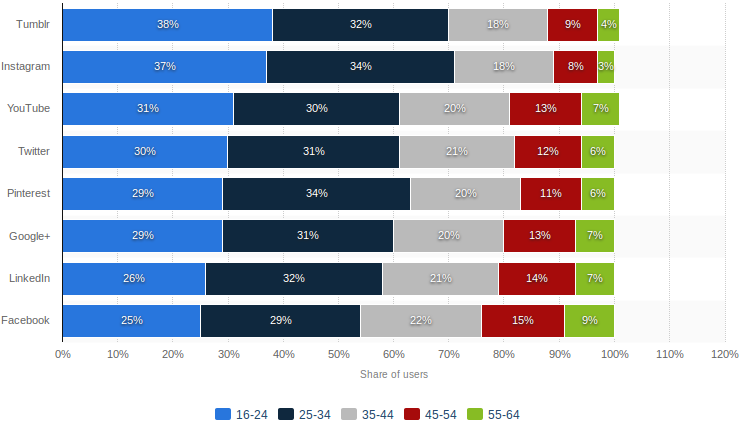
\includegraphics[width=1.0\textwidth]{img/age-distribution.png}
 }
\caption{Distribuzione delle età divisa per Social Network ~\cite{biblio:age_distribution_social}}
\label{img:age_distribution_social}
\end{figure}


L'ultimo obiettivo, invece, servirà ad analizzare un'interazione tra 2 diversi gruppi di utenti, che 
permetterà di studiare il numero di visualizzazioni della notizia in casi più complessi.
Un esempio potrebbe essere quello di voler dividere il numero totale delle persone in due sottoinsiemi così formati:
\begin{itemize}
 \item Il primo gruppo è formato da pochi utenti, tipo il 20\% del totale, ma ogni componente ha un'ottima probabilità di condivisione.
 \item Il secondo gruppo, viceversa, è formato dall'80\% degli utenti, ma ogni componente ha una possibilità minore di condivisione.
\end{itemize}






\section{Progettazione e Implementazione}
\label{section:progettazione}


Per favorire lo studio di un modello che permetta di raggiungere gli obiettivi descritti 
pocanzi, sono state prese le decisioni di seguito elencate.

Si anticipa che il social network verrà astratto ad un grafo scale-free nel quale ogni 
nodo corrisponde ad un utente in possesso di alcune caratteristiche.

Per il primo obiettivo verrà posta l'attenzione su due algoritmi, entrambi impiegati per la creazione di grafi, 
che formano modelli di rete differenti.

Inizialmente verrà mostrato il propagarsi di una notizia in un grafo di tipo 
``Preferential Attachment'' suggerito da Barabási e Albert~\cite{biblio:barabasilab_emergence}.
Le simulazioni proseguiranno poi attraverso un'altra topologia di grafo, sempre scale-free 
con Power Law Degree, descritta però dall'algoritmo di Dorogovtsev e Mendes~\cite{biblio:evolution_networks}.

Il lavoro non parte da dati reali e la scelta di queste topologie di grafi è data 
dalla peculiarità di alcune loro caratteristiche che verranno elencate di seguito:
\begin{itemize}
 \item La topologia di grafo Preferential Attachment si contraddistingue per le seguenti caratteristiche:
 \begin{itemize}
  \item è un modello ampiamente utilizzato per la sua semplicità;
  \item è impiegato in buona parte di studi che trattano argomenti somiglianti lo ``Spreading Rumors'';
  \item non è un grafo di tipo frattale~\cite{biblio:fractal_resistant_disease} ma ha una caratteristica simile. 		%TODO: Lascio la citazione?
 Infatti, non possedendo cricche di almeno 3 nodi, nel momento in cui un nodo non condividesse la notizia, 
 tutti i suoi nodi ``figli'' non riceverebbero mai l'informazione.
 \end{itemize}
 
 \item La topologia di grafo definita da Dorogovtsev e Mendes invece viene descritta come segue:
  \begin{itemize}
  \item è caratterizzata da un modello più complesso;
  \item può avere all'interno del grafo cricche da 3 o più nodi, permettendo così una probabilità maggiore di condivisione della notizia;
  \item è più somigliante\footnote{\scriptsize Non esiste un modello virtuale di una rete sociale reale, 
  bensì ogni ottimizzaziona apportata permette di rendere i risultati delle simulazioni più vicini alla realtà.}
  ad una struttura reale di rete sociale.
 \end{itemize}
\end{itemize}

Cercando di migliorare il modello totale della simulazione è stato deciso di fornire alcune proprietà alla notizia e 
agli utenti(Nodi) che compaiono nella rete sociale.
Mirando al secondo obiettivo risulta necessario fornire alla notizia un ``argomento'' e si 
è così optato per l'inserimento di $N$ valori che definiranno quanto la notizia sia adatta ad per ogni fascia d'età.
Avendo a disposizione la distribuzione delle età, precedentemente mostrata nel grafico di figura~\ref{img:age_distribution_social},
è possibile osservare 5 intervalli di età e quindi è possibile stabilire il valore di $N = 5$.

Risulta ora necessario definire 5 gruppi di utenti per distinguere le differenti età.
Il numero di persone appartenenti ad ogni gruppo verrà definito dalla semplice proporzione:
\[
\frac{N\_NODI\_TOTALI}{100} \cdot \%\_UTENTI\_GRUPPO
\]
dove $\%\_UTENTI\_GRUPPO$ è la percentuale presente nel grafico di figura~\ref{img:age_distribution_social}.

Giunti a questo punto si può constatare come la formula che definisca la probabilità di propagazione 
sia l'unica mancante alla condivisione dell'informazione tra nodo e nodo.
L'idea è quella di dare la ``possibilità'' all'utente di decidere, come nella realtà, se la 
notizia gli interessi i meno. 
Risulta quindi necessario aggiungere all'utente un nuovo paramentro, ovvero l'astensione alla notizia.

Così facendo la notizia verrà condivisa dall'utente \emph{'i-esimo'} con una certa età \emph{'e'} se:
\[
NOTIZIA_e \quad > \quad UTENTE_i.astensione
\]
dove $\quad NOTIZIA_e \quad$ è la forza di condivisione della notizia su una data fascia d'età \emph{'e'}, 
mentre $\quad UTENTE_i.astensione \quad$ è l'astensione alla notizia dell'utente i-esimo.

L'ultimo obiettivo si ri fa su quest'ultima parte appena definita.
Quando si parla di ``forza della notizia'' e di ``forza di astensione'' si vuole considerare un numero tra 0 e 1.
Per ottenere una probabilità di condivisione più o meno alta si agirà solo sulla ``forza di astensione''.
Per come è stata definita la formula della condivisione, sarà sufficiente che la distribuzione dell'astensione sia più 
tendente a 0 per avere una miglior condivisione o, viceversa, più tendente a 1 per avere una minor condivisione.

\subsection{Strumenti}


Dopo aver discusso tutte le fasi della progettazione, si passa ora alla fase della così detta implementazione.

Le simulazioni previste verranno sviluppate in NetLogo che fornisce un ambiente semplice e piuttosto 
personalizzabile nel quale si possano condurre studi in campi differenti.
NetLogo è uno strumento di sviluppo per una programmazione basata ad agenti;
nel lavoro qui presentato gli agenti in questione saranno rappresentati dagli utenti della rete sociale.
Esistono vari simulatori di reti che prevedono una programmazione ad agenti, ma NetLogo,
grazie alla sua semplice sintassi ed una moltitudine di
API\footnote{\scriptsize Application Programming Interface: un insieme di funzionalità utilizzabili dal programmatore
}~\cite{biblio:netlogo_dictionary}fornite dal linguaggio stesso, ha risposto brillantemente alle esigenze implementative. 
NetLogo è stato scelto anche per la facilità con la quale permette di modellare 
un'interfaccia grafica\footnote{\scriptsize Dall’inglese GUI ovvero Graphical User Interface}.



\subsection{Topologie dei grafi}
\label{section:graph_topologies}


Come già annunciato all'inizio di questo capitolo, i modelli di grafo che verranno studiati in questo lavoro
sono due.


\subsubsection{Preferential Attachment}
\label{section:graph_topologies_pa}
Il modello Preferential Attachment, come già esplicato a inizio capitolo, è altamente diffuso e conosciuto.
Tanto da avere una propria API per la creazione nel dizionario di NetLogo. 
La seguente funzione:
\begin{lstlisting}[label=some-code, style=custom_code]
 generate-preferential-attachment turtles links num-nodes
\end{lstlisting}
risiede all'interno dell'estensione ``network'', e invocandola, verrà creato un grafo di \emph{num-nodes} nodi con le proprietà 
del grafo Preferential Attachment. L'algoritmo di PA, implementato in NetLogo, crea per ogni nuovo nodo un solo collegamento. \\
In figura \ref{img:preferential_attachment} si ha una rappresentazione grafica di un grafo con 20 nodi.

\begin{figure}[!ht]
 \centerline{
  \begin{subfigure}[b]{0.4\textwidth}
    \begin{center}
      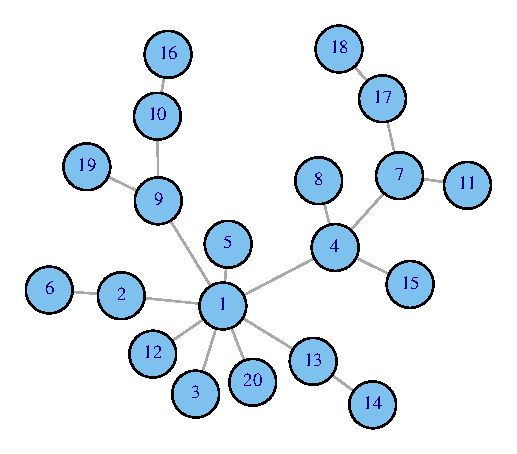
\includegraphics[width=0.75\textwidth]{img/preferential-attachment-graph.eps}
    \end{center}
    \caption{Preferential Attachment}
    \label{img:preferential_attachment}
  \end{subfigure}
  \qquad
  \qquad
  \qquad
  \begin{subfigure}[b]{0.4\textwidth}
    \begin{center}
      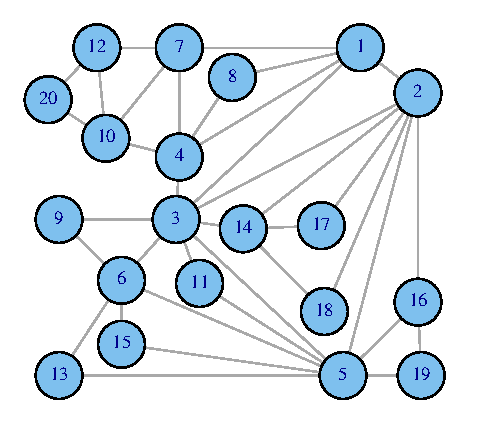
\includegraphics[width=0.75\textwidth]{img/dorogovtsev-mendes-graph.eps}
    \end{center}
    \caption{Dorogovtsev e Mendes}
    \label{img:dorogovtsev_mendes}
  \end{subfigure}
 }
 \caption{Rappresentazione grafica delle due topologie di grafo studiate.}
 \label{img:graph_models}
\end{figure}

\subsubsection{Rete di Dorogovtsev e Mendes}
\label{section:graph_topologies_dm}

\begin{wrapfigure}{r}{0.33\textwidth}
  \vspace*{-25pt}
  \begin{center}
    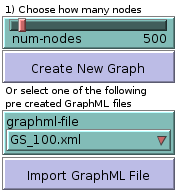
\includegraphics[width=0.28\textwidth]{img/gui-graph.png}
  \end{center}
 \vspace*{-10pt}
 \caption{GUI: Creazione o importazione del grafo}
 \vspace*{-35pt}
 \label{img:gui_graph}
\end{wrapfigure}

Il modello definito da Dorogovtsev e Mendes viene implementato dalla libreria Java chiamata GraphStream~\cite{biblio:graphstream}.
La libreria è formata da tre parti, le seguenti: 
\begin{itemize}
 \item core: Il package principale di GraphStream;
 \item algo: Il package dove vengono implementati tutti gli algoritmi e i generatori della libreria;
 \item ui: Il package che permette la visualizzazione e che da un layout al grafo.
\end{itemize}
I grafi che verranno utilizzati nelle simulazioni sono stati creati da un'applicazione implementata appositamente.
Una volta creati, questi grafi vengono salvati su file in formato GraphML~\cite{biblio:graphml} in modo da 
essere caricati dall'applicativo di NetLogo. \\
In figura \ref{img:dorogovtsev_mendes} è presente una rappresentazione grafica di un grafo con 20 nodi.



\subsection{Inizializzazione del Modello}
\label{section:gui_setup_graph}

\begin{wrapfigure}{l}{0.33\textwidth}
  \vspace*{-35pt}
  \begin{center}
    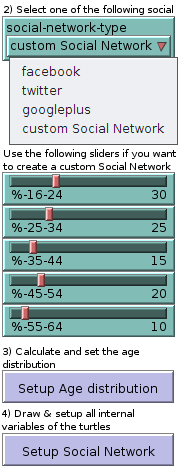
\includegraphics[width=0.28\textwidth]{img/gui-main.png}
  \end{center}
 \vspace*{-10pt}
 \caption{GUI: 
 scelta del Social Netwoks;
 pulsante per il calcolo delle età;
 pulsante per l'inizializzazione dei nodi.}
 \vspace{-15 mm}
 \label{img:gui_main}
\end{wrapfigure}

Al fine di portare a termine gli obiettivi in precedenza descritti è stata creata un'interfaccia grafica 
per permettere all'utilizzatore di interagire con il progetto.
Nella figura~\ref{img:gui_graph} e nella figura~\ref{img:gui_main} vengono mostrate due porzioni di GUI che servono 
all'inizializzazione delle simulazioni.
Nella maggior parte delle dimostrazioni di NetLogo è presente solo un pulsante ``Setup'' 
e un pulsante ``Go''. Data la particolarità del progetto non è stato possibile semplicizzare allo stesso modo 
l'interfaccia grafica; di seguito verranno illustrate le principali caratteristiche grafiche del progetto qui presentato.

In figura~\ref{img:gui_graph} si possono notare due pulsanti:
\begin{itemize}
 \item il primo pulsante permette la creazione di un grafo di tipo Preferential Attachment 
  (Capitolo ~\ref{section:graph_topologies_pa}) con un numero \emph{num-nodes} di nodi.
 \item il secondo pulsante, invece, serve per l'importazione di un file GraphML (Capitolo ~\ref{section:graph_topologies_dm}) tra 
  quelli già creati in precedenza.
\end{itemize}
Dopo aver creato o importato il grafo, viene cercato l'hub della rete, ovvero il nodo con il \emph{degree} più alto.

Un'altra fase necessaria è stata quella dell'importazione nel progetto dei dati di alcuni Social Netwoks
presenti nel grafico di figura~\ref{img:age_distribution_social}.

Nel progetto qui presentato si è scelto di includere i dati dei tre Social Network più popalari, 
essi vengono mostrati in figura ~\ref{img:gui_main}.
In alcune simulazioni si manifesta la necessità di creare condizioni particolari che non possono essere risolte con i dati 
di questi Social Netwok.
Con l'intenzione di rendere l'applicazione più generica possibile, sono stati implementati anche 5 cursori 
che permettono di far selezionare all'utilizzatore parametri personalizzati.
Ognuno dei cinque cursori serve ad impostare la percentuale di utenti facente parte della suddetta fascia d'età e, per
semplicità sono stati chiamati ``\%-\emph{<fascia età inizio>}-\emph{<fascia età fine>}''.

Nell'esempio di figura~\ref{img:gui_main} si può osservarne l'implementazione dove si nota quanto segue.
\begin{itemize}
 \item il gruppo formato di utenti che hanno tra i 16 e i 24 anni rappresenta il 30\%;
 \item il gruppo costituito dalle persone che hanno tra i 25 e i 34 anni sono il 25\%;
 \item il gruppo di persone che hanno tra i 35 e i 44 anni costituisce il 15\%;
 \item le persone che hanno tra i 45 e i 54 anni sono il 20\%;
 \item infine, il gruppo di persone che hanno tra i 55 e i 64 anni sono il 10\%;
\end{itemize}

\begin{wrapfigure}{l}{0.33\textwidth}
  \vspace*{-35pt}
  \begin{center}
    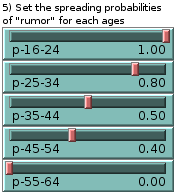
\includegraphics[width=0.28\textwidth]{img/gui-news.png}
  \end{center}
 \vspace*{-10pt}
 \caption{GUI: cursori per personalizzare la notizia.}
 \vspace*{-10pt}
 \label{img:gui_news}
\end{wrapfigure}
Per calcolare la percentuale necessaria di utenti per ogni intervallo di età è necceasio premere il pulsante ``Setup Age Distribution''.
Verrà creato così un vettore grande come il numero dei nodi del grafo, e al suo interno, saranno inseriti gli indici dei 5 gruppi nella 
quantità prevista dalle percentuali. 
Questo procedimento farà si che ogni nodo del grafo avrà un suo preciso valore nell'array, 
di modo da far sì che si identifichi il gruppo di appartenenza.
Il pulsante ``Setup Social Netwoks'', invece, serve a eseguire il reset dei dati base degli utenti, riportando la simulazione 
allo stato iniziale, senza eliminare nè il grafo nè il vettore delle ``età''.
Col temine ``stato iniziale della simulazione'' si intende l'inserimento della notizia nell'hub, in modo da farlo 
diventare il primo ``Spreader''; intanto gli altri nodi del grafo saranno etichettati come 
``Ignorant'' e, per ciascuno, sarà calcolato un nuovo valore di astensione alla notizia.

\begin{wrapfigure}{r}{0.33\textwidth}
  \vspace*{-40pt}
  \begin{center}
    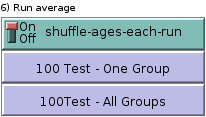
\includegraphics[width=0.28\textwidth]{img/gui-first-second-test.png}
  \end{center}
 \vspace*{-10pt}
 \caption{GUI: 
 pulsanti per dare il via ai primi due test}
 \vspace*{-10pt}
 \label{img:gui_first_second_test}
\end{wrapfigure}
Esistono altri 5 cursori, mostrati in figura~\ref{img:gui_news}, i quali identificano l'intensità con la quale la notizia 
è importante verso un certo gruppo di utenti. 
La definizione\\
``p-\emph{<fascia età inizio>}-\emph{<fascia età fine>}'' si utilizza per indicare la probabilità di condivisione della notizia 
in una particolare fascia d'età.
Nell'esempio in figura~\ref{img:gui_news} la probabilità nel primo gruppo vale 1.0, ovvero la condivisione avrà \emph{sempre} esito positivo.
Nel quinto gruppo si ha, al contrario, probabilità nulla, pari a 0 e la condivisione non andrà mai a buon fine. 
Nei casi intermedi, invece, viene confrontato il valore di astensione dell'utente col valore del cursore dell'età dell'utente
come è stato definito in fase di progettazione (Capitolo ~\ref{section:progettazione}).
I pulsanti presenti in figura~\ref{img:gui_first_second_test} servono a dare il via al test del primo e secondo obiettivo.

\subsection{Sviluppo delle Simulazioni}
Oltre all'inizializzazione della rete e alla configurazione dei suoi agenti, è stata progettata un'architettura in grado di
soddisfare gli obiettivi prefissati.

%Anche per questa fase sono stati inseriti dei pulsanti che danno la possibilità di avviare le simulazioni.


\subsubsection{Propagazione della Notizia}
L'algoritmo~\ref{alg:core_spread}, data la sua importanza, è stato definito il nucleo delle simulazioni 
ed è colui che calcola, ad ogni passo, come la notizia si propaghi. 

\vspace*{-10pt}
\begin{algorithm}
 \begin{algorithmic}[1]
    \Procedure{Core}{$nodes, news$}
      \If {(all nodes have seen the news)}
	\State \Return END\smuscore OK
      \Else 
	\ForAll {(node \textbf{in} nodes \textbf{with} [seen\smuscore news = \textbf{false}])}
	  \If {(\textbf{any} node$_{neighbors}$ \textbf{with} [shared\smuscore news = \textbf{true}])}\\
	  
	    \Comment{Leggo il valore di probabilità della notizia per l'età del utente corrente}
	    \State p\smuscore news $\gets$ news$_{prob[node_{age}]}$
	    
	    \If { p\smuscore news $\geq$ node.chance\smuscore of\smuscore abstention }
	      \State node$_{tmp\smuscore shared\smuscore news} \gets$ \textbf{true}
	    \EndIf
	    \State node$_{tmp\smuscore seen\smuscore news} \gets$ \textbf{true}
	    
	  \EndIf
	\EndFor
	\If {(\textbf{no} nodes \textbf{with} [tmp\smuscore seen\smuscore news = \textbf{True}])}
	  \State \Return END\smuscore KO
	\EndIf
	
	\ForAll {(node \textbf{in} nodes \textbf{with} [tmp\smuscore seen\smuscore news = \textbf{true}])}
	  \State node$_{seen\smuscore news} \gets$ \textbf{true}
	  \State node$_{tmp\smuscore seen\smuscore news} \gets$ \textbf{false}
	\EndFor
	
	\ForAll {(node \textbf{in} nodes \textbf{with} [tmp\smuscore shared\smuscore news = \textbf{true}])}
	  \State node$_{shared\smuscore news} \gets$ \textbf{true}
	  \State node$_{tmp\smuscore shared\smuscore news} \gets$ \textbf{false}
	\EndFor
      
	\State \Return SIMULATION\smuscore NOT\smuscore FINISHED\smuscore YET
      \EndIf
    \EndProcedure
 \end{algorithmic}
 
 \caption{Nucleo della propagazione della notizia}
 \label{alg:core_spread}
\end{algorithm}
 \vspace*{-10pt}
La funzione Core prima verifica se ci sia qualche nodo che non ha visualizzato la notizia (Riga 2), 
poi richiede a tutti i nodi ``Ignorants'' se hanno un vicino ``Spreader'' (Riga 5 e 6). 
Nel caso in cui questa ipotesi sia soddisfa, viene letta la probabilità della notizia rispetto all'età del 
nodo ``Ignorant'' corrente (Riga 8) e viene eseguito il confronto con il valore di astensione alla notizia (Riga 9), 
come stabilito in fase di progettazione descritta nel capitolo~\ref{section:progettazione}. 
Inoltre esiste un'altra funzione, altrettanto importante, che si occupa di calcolare la media di $N$ test del numero di ``Viewers''.
Ad ogni esecuzione, però, la funzione si preoccupa anche di effettuare il reset di tutti gli agenti presenti nella simulazione.
Essa calcola nuovamente un valore di astensione per ogni nodo e, se richiesto, rimescola gli elementi del 
vettore contenente le differenti età al fine di avere ampia casualità nei test effettuati.

\subsubsection{``100 Test - One Group''}
Questo pulsante viene premuto per eseguire la prima simulazione. 
Come prima azione verrà impostato il Social Netwok di tipo ``custom'', esso permetterà di poter personalizzare
la percentuale di utenti nei 5 gruppi, impostando il 100\% nel primo gruppo e 0\% negli altri gruppi. 

Successivamente il test eseguirà la procedura di propagazione della notizia facendo variare la probabilità 
della notizia per il primo gruppo, quindi il cursore ``p-16-24'', da 0 a 1 con passi di 0.05.
Il risultato sarà un grafico che mostrerà sull'asse X i ticks, ovvero l'avanzamento della simulazione, quindi la forza della notizia; 
mentre sull'asse Y ci sarà la media di 100 test del numero di ``Viewers''.

\subsubsection{``100 Test - All Groups''}
La seconda simulazione utilizza invece le percentuali di utenti definite nel grafico della statistica di figura~\ref{img:age_distribution_social},
facendo variare una delle probabilità della notizia da 0 a 1 con step di 0.05.
Inzialmente si studierà cosa capita al solo variare della forza della notizia del gruppo più numeroso; 
successivamente verrà invece analizzato il comportamento della rete al variare della forza della notizia di tutti i gruppi.
Così facendo si otterrà un grafico dove sull'asse X ci saranno nuovamente i ticks, ovvero l'avanzamento della simulazione, quindi 
la forza della notizia, mentre sull'asse Y ci saranno tutte le medie di 500 test del numero di ``Viewers'' di ogni gruppo.

\begin{wrapfigure}{r}{0.30\textwidth}
  \vspace*{-35pt}
  \begin{center}
    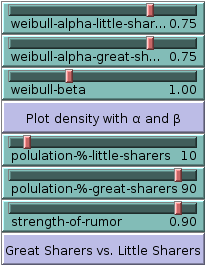
\includegraphics[width=0.28\textwidth]{img/gui-third-test.png}
  \end{center}
 \vspace*{-10pt}
 \caption{GUI: terzo test}
 \vspace*{-20pt}
 \label{img:gui_third_test}
\end{wrapfigure}



\subsubsection{``Great Sharers vs. Little Sharers''}
\label{section:great_sharers_vs_little_sharers}

L'ultima simulazione è quella che si distingue di più dalle altre considerato il concetto su cui si basa;
si vuole infatti studiare il confronto tra due gruppi che, a differenza dei precedenti test, si distinguono 
per la loro probabilità di astensione alla divulgazione della notizia. 
Nelle prime due simulazioni questo dato veniva stabilito da una funzione random caratterizzata da una distribuzione di
densità lineare.
In questo test, invece, l'astensione alla condivisione viene calcolata tramite una funzione di distribuzione di probabilità non lineare; 
quella scelta è la funzione Weibull\cite{biblio:weibull}.
La funzione ``random-weibull'' fa variare la densità della distribuzione per mezzo di due parametri $\alpha$ e $\beta$.
Il valore restituito dalla funzione è sempre un numero tra 0 ed 1 perciò, per il calcolo della propagazione della notizia,
può essere riutilizzato l'algoritmo~\ref{alg:core_spread} mostrato in precedenza.
In figura~\ref{img:gui_third_test} sono presenti 3 slider per la manipolazione degli $\alpha$ e di $\beta$. 
Il paramentro $\alpha$ modifica la pendenza della curva mentre il paramentro $\beta$ modifica sopratutto la forma della curva.
Per la simulazione ci serviremo di due cursori per la manipolazione del paramentro $\alpha$ dei due gruppi.
In figura~\ref{img:weibull_alpha_0_75} viene mostrato il dislivello a cui si è appena fatto riferimento.
Nel primo istogramma, con $X$ più densa vicino a 0, viene permessa una miglior condivisione mentre nel secondo grafico ne risulta una peggiore.


\begin{figure}[!htb]
\centerline {
  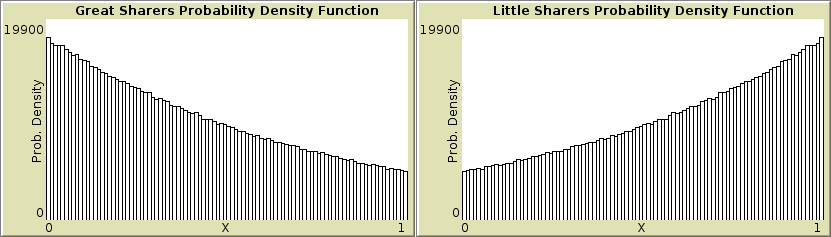
\includegraphics[width=1.1\textwidth]{img/weibull-alpha-0.75.png}
}
\caption[caption for img/weibull-alpha-0.75.png]{I due istogrammi mostrano la rappresentazione di un vettore $X$ di 1 milione di cifre 
calcolato mediante la funzione di densità di probabilità Weibull, con $\alpha = 0.75$.
Il grafico di sinistra rappresenta la distribuzione originale, 
mentre quello di destra la sua \emph{quasi \protect\footnotemark} speculare calcolata grazie: $\forall x \in X, \quad 1 - x$.}
\label{img:weibull_alpha_0_75}
\end{figure}
\footnotetext{\scriptsize Quando si parla di numeri random non è possibile pretendere di ottenere lo stesso identico comportamento.} 

In figura~\ref{img:gui_third_test} sono presenti altri 2 cursori per definire la percentuale degli utenti appartenenti ad ogni gruppo e 
il cursore per impostare la ``forza'' della notizia.
Alla pressione del tasto ``Great Sharers vs. Little Sharers'' viene lanciata una simulazione che riguarda i parametri selezionati.
Vista la quantità di test da fare con tutti le combinazioni di parametri possibili è stata scritta una procedura\footnote{\scriptsize 
La procedura che permette di elaborare tutti i test impiega un tempo prolungato per la sua esecuzione.
Per invocarla è sufficiente inserire il comando ``great-sharers-in-comparison-to-little-sharers-all-tests'' in modalità \emph{Observer} nel \emph{Command Center} di NetLogo.
} che, grazie ai sui tre cicli annidati, riesce a considerare tutte le possibilità richieste dal terzo obiettivo.
L'algoritmo \ref{alg:third_test} mostra su quali parametri agiscono i tre cicli.

Il primo ciclo, più esterno, itera su alcuni valori di forza della notizia, 
ovvero i seguenti: $0.50 \quad 0.60 \quad 0.70 \quad 0.75 \quad 0.80 \quad 0.90$.\\
Il secondo ciclo, quello centrale, modifica il numero di individui per ogni gruppo. 
Ad ogni passo viene incrementato il numero di persone con un'alta possibilità di condivisione 
passando dal 10\% al 90\%. Operazione inversa a quella appena descritta viene eseguita per le persone con bassa possibilità di 
condivisione passando dal 90\% al 10\% della popolazione totale.
Il terzo ciclo, più interno, invece itera sul parametro $\alpha$ modificando quindi la pendenza della 
curva per gli individui con alta probabilità di condivisione.
Come si può notare il paramentro $\alpha$ del gruppo che condivide meno viene preso in ingresso dalla funzione e
mai manipolato.

\begin{algorithm}
 \begin{algorithmic}[1]
    \Procedure{third-test-all}{alpha\smuscore little\smuscore sharers}
      \State weibull\smuscore alpha\smuscore little\smuscore sharers  $\gets$ alpha\smuscore little\smuscore sharers
      \ForAll {(news\smuscore strength \textbf{in} [0.50 0.60 0.70 0.75 0.80 0.90])}
	\State population\smuscore \%\smuscore step $\gets$ 10
	\While {(population\smuscore \%\smuscore step $\leq$ 90)}
	  \State \%\smuscore little\smuscore sharers  $\gets$  (100 - population\smuscore \%\smuscore step)
	  \State \%\smuscore great\smuscore sharers  $\gets$  population\smuscore \%\smuscore step
	  
	  \ForAll {(weibull\smuscore alpha\smuscore great\smuscore sharers \textbf{in} [0.25 0.50 0.75 1.0])}
	  
	    \Comment Eseguo la simulazione 500 volte con i paramentri correnti per avere un risultato mediato più valido possibile
	  
	  \EndFor
	  
	  \State population\smuscore \%\smuscore step $\gets$ population\smuscore \%\smuscore step + 5
	  
	\EndWhile
      \EndFor
    \EndProcedure
 \end{algorithmic}
 
 \caption{Tre cicli annidati per considerare tutte le possibilità interessanti del terzo obiettivo}
 \label{alg:third_test}
\end{algorithm}


\newpage
\section{Analisi dei Risultati}
\label{section:analisirisultati}

%1 test: Questa proprietà lo penalizza nelle simulazioni che sono 





In quest'ultima analisi, invece, verrà mostrata un'interazione tra 2 diversi gruppi di utenti (Nodi).
Il primo gruppo è formato da persone con un'alta probabilità di condividere la notizia 
mentre nel secondo, al contrario, da persone con una bassa probabilità.
Questo studio punta ad analizzare quante visualizzazioni vengono fatte per una singola informazione condivisa.
Verrà anche condotto uno studio in cui il totale degli utenti si divide in due gruppi costituiti da, ad esempio, 
pochi utenti con alte probabilità di condividere l'informazione e, viceversa, 
molti utenti con basse probabilità di condivisione.
La possibilità di condivisione è data nuovamente dal confronto tra 
la ``forza della notizia'' e la ``forza di astensione''\ref{subsection:TODO}. 
In questo caso, però, l'astensione viene calcolata tramite una funzione di distribuzione di probabilità non lineare,
quella scelta è la funzione Weibull.
La funzione ``random-weibull''\ref{subsection:TODO} fa variare, per mezzo dei due parametri $\alpha$ e $\beta$, la pendenza della distribuzione
e, di conseguenza, anche la sua densità.

Per ottenere una curva di distribuzione più o meno inclinata, in seguito ai tentativi attuati, 
è stato ritenuto opportuno mantenere il valore di $\beta$ costante a 1.0 e variare, invece, quello di $\alpha$.


\begin{figure}[!ht]
\centerline {
  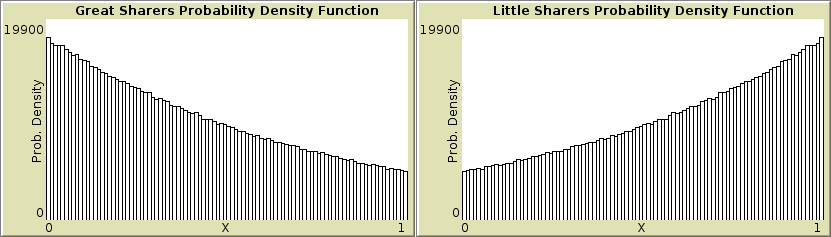
\includegraphics[width=1.1\textwidth]{img/weibull-alpha-0.75.png}
}
\caption{I due istogrammi mostrano la rappresentazione di un vettore $X$ di 1 milione di cifre 
calcolato mediante la funzione di densità di probabilità Weibull, con $\alpha = 0.75$.
Il grafico di sinistra rappresenta la distribuzione originale, 
mentre quello di destra la sua speculare calcolata grazie: $\forall x \in X, \quad 1 - x$.}
\label{img:weibull_alpha_0_75}
\end{figure}

Nella fig.\ref{img:weibull_alpha_0_75} il dislivello non è troppo alto e questo permette 
comunque al gruppo 2 un buon grado di condivisione della notizia.

Questa analisi è stata sviluppata mediante tre cicli annidati che hanno considerato tutte le 
possibilità che verranno di seguito esposte.\\
Il primo ciclo più esterno itera su alcuni valori di forza della notizia, 
ovvero i seguenti: $0.50 \quad 0.60 \quad 0.70 \quad 0.75 \quad 0.80 \quad 0.90$.\\
Il secondo ciclo, quello centrale, modifica il numero di individui per ogni gruppo. 
Ad ogni passo viene incrementato il numero di persone con un'alta possibilità di condivisione 
passando dal 10\% al 90\%. Operazione inversa viene eseguita per le persone con bassa possibilità di 
condivisione passando dal 90\% al 10\% della popolazione totale.
Il terzo ciclo, più interno, invece itera sul parametro $\alpha$ modificando quindi la pendenza della 
curva per gli individui con alta probabilità di condivisione.

Il test viene composto da i parametri dinamici appena citati e dai seguenti parametri statici:
\begin{itemize}
\item La dimensione della popolazione non cambia mai e resta sempre di 500 Nodi;
\item Il parametro $\alpha$ del gruppo con bassa probabilità di condivisione rimane $0.75$, 
ottenendo una densità di probabilità come in figura \ref{img:weibull_alpha_0_75};
\item La topologia del grafo è la stessa per ogni esecuzione del test;
\end{itemize}

Il risultato di ogni test inoltre viene mediato sull'esito di 500 test.

La figura \ref{img:last_test_str_0_5} mostra il risultato atteso, 
ovvero la crescita del numero di visualizzazioni sia al variare di $\alpha$ che all'aumentare 
dei nodi con alta probabilità di condivisione.

Si vuole inoltre porre l'attenzione su come con un valore di $\alpha$ 
molto basso ($0.2$) ed un numero di nodi con alta probabilità di condivisione pari a 150 corrisponda 
a ~ 300 visualizzazioni totali, quasi le stesse ottenute da un valore di $\alpha$ = 1.0 e 325 nodi con 
alta probabilità di condivisione.




\begin{figure}[!ht]
\centerline {
  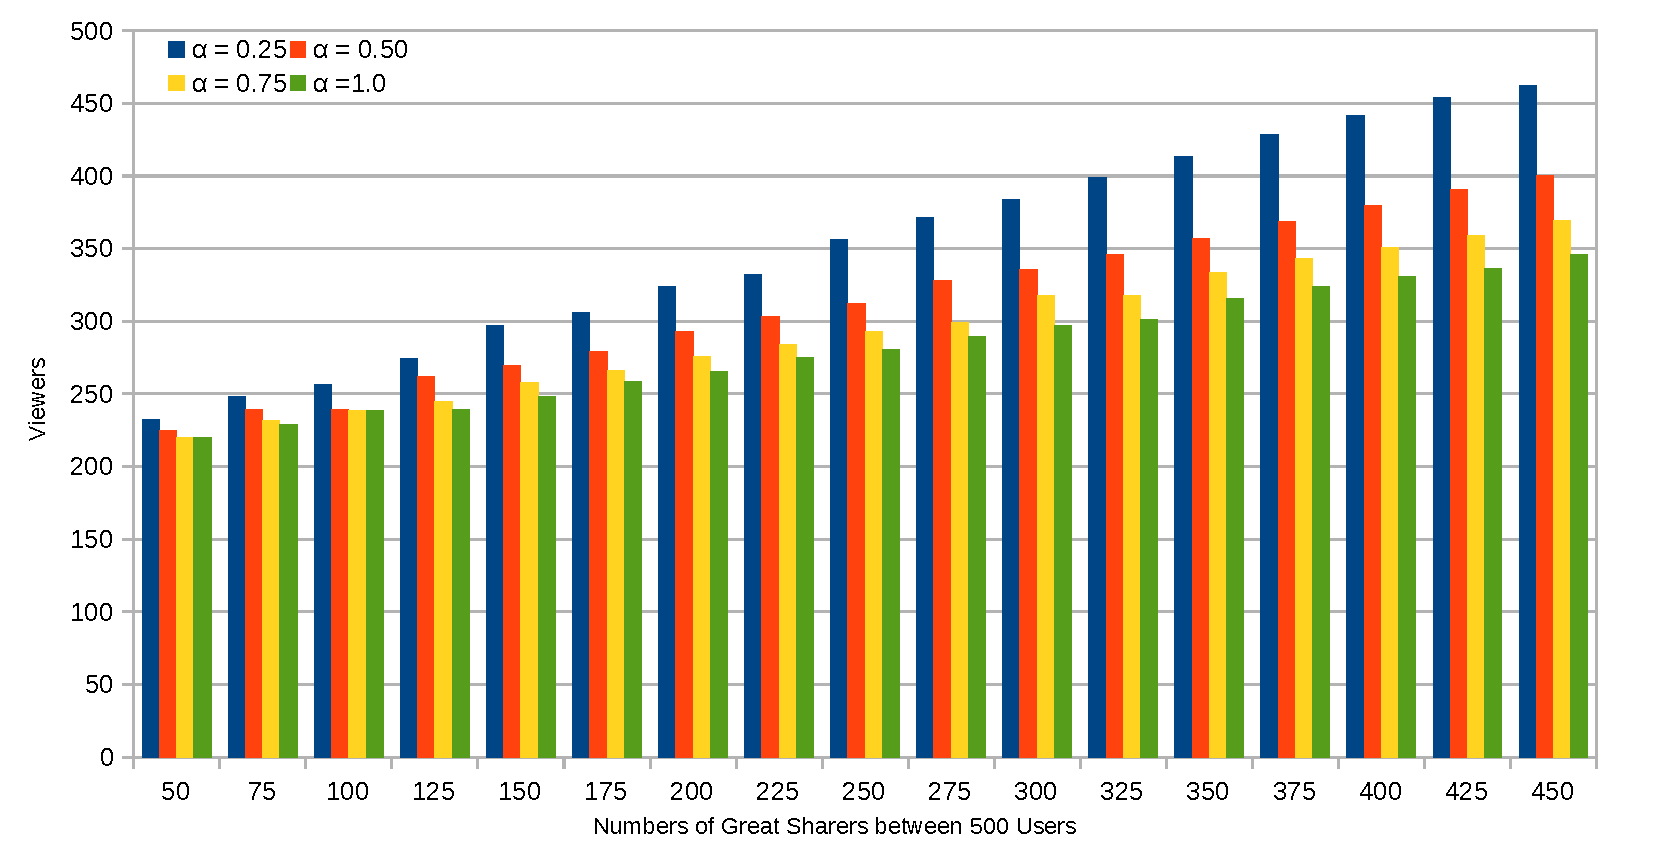
\includegraphics[width=1.1\textwidth]{charts/last-test-str_0.5.pdf}
}
\caption{Grafico del risultato dell'ultimo test con forza della notizia pari a $0.50$, 
500 nodi totali e $\alpha$ del gruppo con bassa probabilità di condivisione = $0.75$}
\label{img:last_test_str_0_5}
\end{figure}












\section{Conclusioni}
\label{section:conclusioni}

In conclusione i risultati posti come obiettivo sono stati raggiunti.

Innanzitutto è stato studiato quale modello di grafo fosse più in linea con il tipo di 
analisi che questo progetto tratta.
La topologia di grafo proposta da Dorogovtsev e Mendes ha avuto risultati di condivisione migliori. 
Il parametro chiave è definito dalla sua struttura particolare che 
prevede un numero di connessioni quasi doppio rispetto al Preferential Attachment.

Il secondo studio invece ha fornito una risposta concreta a come una informazione con un certo argomento 
viene condivisa in un Social Network con differenti utenti.
L'argomento viene ``deciso'' tramite 5 valori che vanno ad incidere sulla probabilità di condivisione della notizia.
Si può affermare che, più la notizia ha importanza, più questa viene condivisa.
I test effettuati non sono stati esaustivi, ma sono bastati per capire la tendenza appena affermata.
Effettuare tutti i test sarebbe stato poco produttivo e avrebbe impiegato un'enormità di risorse.
Si vuol far notare infatti che per affrontare tutte le possibilità, dati i 5 parametri, ci sarebbero volute
\[
  \left(\frac{1 - 0}{0.05}\right)^5 * 500 test = 1.600.000.000
\]
simulazioni complete per garantire la stessa precisione. 

Per quanto concerne il terzo studio, sono stati confrontati due gruppi di utenti con differenti 
proprietà di astensione alla notizia. Queste proprietà sono state descritte dalla funzione di probabilità 
Weibull che, grazie ad un parametro $\alpha$, permette di modificare la densità della distribuzione.
Così facendo si avrà un gruppo con una probabilità di condivisione maggiore dell'altro.
Nel test effettuato è stato mostrato un nuovo risultato. 
La forza della notizia in questo caso non influisce con la crescita dei ``Viewers''.
Il parametro importante è l'aumentare degli individui con la bassa astensione alla notizia rispetto a quelli
con una più alta.
Si pone anche l'attenzione come, in alcuni casi, pochi utenti che condividono molto possono avere un'influenza 
maggiore di tanti che condividono meno.


\subsection{Sviluppi Futuri}

Come già affermato nell'introduzione, questo lavoro è stato già affrontato in passato e continuerà ad
esserlo dato l'importanza che, l'argomento discusso, ha nella società moderna.



%Come abbiamo potuto osservare sono pienamente in linea con 
% motivare il singolo grafo



Prendere i risultati del 3\degree test e confrontarli con quelli dei test base e vedere come si comportano, minore? maggiore?





















\newpage

\newpage
\begin{thebibliography}{5}


%First rumor paper found
\bibitem{biblio:stochastic_rumours} 
D. J. Daley, D. G. Kendall.\\
\emph{Stochastic Rumours}.\\
\url{http://imamat.oxfordjournals.org/content/1/1/42.abstract}\\

\bibitem{biblio:barabasilab_emergence}
A.-L. Barabási, R. Albert.\\
\emph{Emergence of scaling in random networks}\\
\url{http://www.barabasilab.com/pubs/CCNR-ALB_Publications/199910-15_Science-Emergence/199910-15_Science-Emergence.pdf}\\

\bibitem{biblio:evolution_networks}
S. N. Dorogovtsev, J. F. F. Mendes.\\
\emph{Evolution of networks}\\
\url{http://arxiv.org/pdf/cond-mat/0106144v2.pdf}\\

\bibitem{biblio:age_distribution_social}
Statista 2015.\\
\emph{Age distribution of active social media users worldwide as of 3rd quarter 2014, by platform }.\\
\url{http://www.statista.com/statistics/274829/age-distribution-of-active-social-media-users-worldwide-by-platform/}\\

\bibitem{biblio:fractal_resistant_disease} 
Zhongzhi Zhang, Shuigeng Zhou, Tao Zou, Guisheng Chen.\\
\emph{Fractal scale-free networks resistant to disease spread}.\\
\url{http://arxiv.org/pdf/0804.3186.pdf}\\

\bibitem{biblio:netlogo_dictionary} 
http://ccl.northwestern.edu.\\
\emph{NetLogo Dictionary}.\\
\url{http://ccl.northwestern.edu/netlogo/docs/dictionary.html}\\

\bibitem{biblio:graphstream} 
GraphStream Team\\
\emph{GraphStream Project}.\\
\url{http://graphstream-project.org/}\\

\bibitem{biblio:graphml} 
GraphML Team\\
\emph{The GraphML File Format}.\\
\url{http://graphml.graphdrawing.org/}\\

\bibitem{biblio:spread_rumor}
Nick Fedewa, Emily Krause, Alexandra Sisson and Advisor: James Angelos.\\
\emph{Spread of A Rumor}.\\
\url{http://www.siam.org/students/siuro/vol6/S01182.pdf}\\


\end{thebibliography}

\end{document}